% Companion P: Pion Decay as Hadron→Lepton Injection Test
% EDC Paper 3 Series — Companion Document
% Version: 0.3 (internal QA hardened)
% Date: 2026-01-20

\documentclass[11pt,a4paper]{article}

% ============================================================
% FONT CONFIGURATION (with fallback for system compatibility)
% ============================================================
\usepackage{fontspec}
\IfFontExistsTF{TeX Gyre Termes}{%
  \setmainfont{TeX Gyre Termes}
}{%
  \setmainfont{Times New Roman}[Ligatures=TeX]
}

% ============================================================
% STANDARD PACKAGES
% ============================================================
\usepackage{amsmath,amssymb,amsthm}
\usepackage{geometry}
\usepackage{hyperref}
\usepackage{cleveref}
\usepackage{booktabs}
\usepackage{enumitem}
\usepackage{xcolor}
\usepackage{tcolorbox}  % Required for edc_style.tex
\usepackage{tikz}
\usetikzlibrary{arrows.meta,positioning,decorations.pathmorphing,shapes.geometric}

% Load shared EDC style (includes theorem environments)
% edc_style.tex — Canonical EDC Paper Style for Paper 3 Series
% Version 1.0 — 2026-01-20
%
% USAGE: Include in preamble AFTER loading packages but BEFORE \begin{document}
%   % edc_style.tex — Canonical EDC Paper Style for Paper 3 Series
% Version 1.0 — 2026-01-20
%
% USAGE: Include in preamble AFTER loading packages but BEFORE \begin{document}
%   % edc_style.tex — Canonical EDC Paper Style for Paper 3 Series
% Version 1.0 — 2026-01-20
%
% USAGE: Include in preamble AFTER loading packages but BEFORE \begin{document}
%   \input{../_shared/style/edc_style}
%   \input{../_shared/style/tikz_style_edc}  % if using TikZ figures
%
% REQUIRED PACKAGES (load these in main document before \input):
%   fontspec, amsmath, amssymb, amsthm, mathtools, geometry
%   hyperref, enumitem, booktabs, array, xcolor, tcolorbox
%
% ============================================================

% ============================================================
%  EPISTEMIC TAG COLORS
% ============================================================
\definecolor{tagDer}{RGB}{0,128,0}      % Green - Derived
\definecolor{tagDc}{RGB}{0,0,200}       % Blue - Deduced/Constrained
\definecolor{tagCal}{RGB}{200,0,0}      % Red - Calibrated
\definecolor{tagP}{RGB}{128,0,128}      % Purple - Postulated
\definecolor{tagBL}{RGB}{128,128,128}   % Gray - Baseline
\definecolor{tagI}{RGB}{255,140,0}      % Orange - Identified
\definecolor{tagOpen}{RGB}{200,100,0}   % Dark orange - Open

% ============================================================
%  EPISTEMIC TAG COMMANDS
% ============================================================
% Use these to mark claims with their epistemic status
\newcommand{\tagDer}{\textcolor{tagDer}{\textbf{[Der]}}}    % Derived from axioms
\newcommand{\tagDc}{\textcolor{tagDc}{\textbf{[Dc]}}}       % Deduced/Constrained
\newcommand{\tagCal}{\textcolor{tagCal}{\textbf{[Cal]}}}    % Calibrated (fitted)
\newcommand{\tagP}{\textcolor{tagP}{\textbf{[P]}}}          % Postulated
\newcommand{\tagBL}{\textcolor{tagBL}{\textbf{[BL]}}}       % Baseline (external fact)
\newcommand{\tagI}{\textcolor{tagI}{\textbf{[I]}}}          % Identified (pattern match)
\newcommand{\tagOpen}{\textcolor{tagOpen}{\textbf{[OPEN]}}} % Open problem
\newcommand{\tagDef}{\textcolor{tagDc}{\textbf{[Def]}}}     % Definition

% ============================================================
%  THEOREM ENVIRONMENTS
% ============================================================
\newtheorem{postulate}{Postulate}
\newtheorem{definition}{Definition}[section]
\newtheorem{theorem}{Theorem}[section]
\newtheorem{lemma}[theorem]{Lemma}
\newtheorem{corollary}[theorem]{Corollary}
\newtheorem{proposition}[theorem]{Proposition}
\newtheorem{remark}{Remark}[section]

% ============================================================
%  COMMON EDC SYMBOLS
% ============================================================
% Symmetry groups
\newcommand{\Ztwo}{\mathbb{Z}_2}
\newcommand{\Zthree}{\mathbb{Z}_3}
\newcommand{\Ztri}{\mathbb{Z}_3}    % alias
\newcommand{\Zsix}{\mathbb{Z}_6}

% Geometric objects
\newcommand{\Sthree}{S^3}           % 3-sphere
\newcommand{\Stwo}{S^2}             % 2-sphere
\newcommand{\Bthree}{B^3}           % 3-ball
\newcommand{\Mfive}{\mathcal{M}_5}  % 5D manifold
\newcommand{\Bfour}{\mathcal{B}_4}  % 4D brane

% Physical quantities
\newcommand{\tension}{\tau}         % string/flux-tube tension (E/L)
\newcommand{\re}{r_e}               % electron radius

% Operators
\newcommand{\Pfrozen}{\mathcal{P}_{\mathrm{frozen}}}  % Frozen projection operator
\newcommand{\Ebrane}{\mathcal{E}_{\mathrm{brane}}}    % Brane energy store

% Bulk-brane exchange current (canonical notation from Framework v2.0)
\newcommand{\Jbb}[1]{J^{#1}_{\mathrm{bulk}\to\mathrm{brane}}}

% ============================================================
%  TCOLORBOX STYLES FOR EDC PAPERS
% ============================================================
% Cornerstone box (blue) — key claims/foundations
\tcbset{
    edcCornerstone/.style={
        colback=blue!5,
        colframe=blue!40!black,
        fonttitle=\bfseries
    }
}

% Guardrail box (gray) — epistemic warnings/constraints
\tcbset{
    edcGuardrail/.style={
        colback=gray!5!white,
        colframe=gray!60!black,
        fonttitle=\bfseries
    }
}

% PPN box (blue, lighter) — Physical Process Narrative
\tcbset{
    edcPPN/.style={
        colback=blue!5,
        colframe=blue!50!black,
        fonttitle=\bfseries
    }
}

% Canonical box (yellow/orange) — canonical definitions/glossary
\tcbset{
    edcCanonical/.style={
        colback=yellow!5,
        colframe=orange!60!black,
        fonttitle=\bfseries
    }
}

% Conceptual box (yellow/orange, lighter) — conceptual pictures
\tcbset{
    edcConcept/.style={
        colback=yellow!5,
        colframe=orange!50!black,
        fonttitle=\bfseries
    }
}

% Pathway box (purple) — energy pathways, mechanisms
\tcbset{
    edcPathway/.style={
        colback=purple!5,
        colframe=purple!40!black,
        fonttitle=\bfseries
    }
}

% Model box (green) — mechanical analogies, heuristics
\tcbset{
    edcModel/.style={
        colback=green!5,
        colframe=green!40!black,
        fonttitle=\bfseries
    }
}

% Warning box (red) — non-overclaim, limitations
\tcbset{
    edcWarning/.style={
        colback=red!5,
        colframe=red!40!black,
        fonttitle=\bfseries
    }
}

% Framework quote box (gray) — verbatim from Framework v2.0
\tcbset{
    edcFramework/.style={
        colback=gray!5!white,
        colframe=gray!60!black,
        fonttitle=\small
    }
}

% Mechanism box (teal) — mechanistic dimension principle narrative
\tcbset{
    edcMechanism/.style={
        colback=teal!5,
        colframe=teal!50!black,
        fonttitle=\bfseries,
        title={Mechanistic Dimension Note (Canon)}
    }
}

% ============================================================
%  MECHANISTIC DIMENSION HELPER MACRO
% ============================================================
% Usage: \edcMechanismNote{bulk cause}{brane process}{3D output}
%
% Example:
%   \edcMechanismNote{Junction relaxes toward Steiner minimum}%
%                    {Energy pumps into brane-layer modes, redistributes}%
%                    {Electron, antineutrino, proton emerge on 3D side}
%
\newcommand{\edcMechanismNote}[3]{%
\begin{tcolorbox}[edcMechanism]
\begin{itemize}[nosep,leftmargin=*]
    \item \textbf{5D cause (bulk):} #1
    \item \textbf{Brane-layer process:} #2
    \item \textbf{3D observation (output):} #3
\end{itemize}
\vspace{0.3em}
\footnotesize\textit{Ledger closure must hold: bulk + brane + 3D outputs conserve energy/quantum numbers.}
\end{tcolorbox}
}

% ============================================================
%  RELATED DOCUMENTS MACRO
% ============================================================
% Usage: \edcRelatedDocs{main paper title}{main DOI}{companion list}
%
% Example:
%     A: \emph{Effective Lagrangian} (\href{...}{DOI}) $\cdot$
%     B: \emph{WKB Prefactor} (\href{...}{DOI})
%   }

% NOTE: \edcRelatedDocs macro deprecated (DOI registry consolidated)
% Use consolidated Zenodo article as primary reference instead.

% ============================================================
%  DOI REGISTRY DEPRECATED
% ============================================================
% Previous individual DOIs have been deprecated.
% All EDC Weak Sector content is now consolidated into a single
% Zenodo article. See paper_3_series/19_edc_weak_sector_zenodo_article/

% ============================================================
%  PHYSICAL NARRATION RULE REMINDER
% ============================================================
% Every key equation MUST be accompanied by a physical narrative stating:
%   1. 5D cause: What changes in the bulk-core configuration?
%   2. Brane response: How does the brane absorb/redistribute energy?
%   3. 3D observable output: What do observers detect on the 3D side?
%
% This rule eliminates "numerology smell" by ensuring every formula
% has a mechanistic interpretation.

% ============================================================
%  END OF STYLE FILE
% ============================================================

%   % tikz_style_edc.tex — Reusable TikZ styles for EDC papers
% Version 1.0 — 2026-01-20
% Include via: \input{tikz_style_edc}

% ============================================================
% REQUIRED LIBRARIES (must be loaded in main document)
% ============================================================
% \usetikzlibrary{calc,angles,quotes,decorations.markings,decorations.pathmorphing,positioning}

% ============================================================
% POSITIONING DEFAULTS
% ============================================================
\tikzset{
    % Default node distances for horizontal/vertical layouts
    edc node distance/.style={node distance=1.6cm and 2.0cm},
    % Compact variant for dense diagrams
    edc compact/.style={node distance=1.2cm and 1.5cm},
    % Spread variant for clarity
    edc spread/.style={node distance=2.0cm and 2.5cm},
}

% ============================================================
% COLOR PALETTE (consistent with epistemic tags)
% ============================================================
\definecolor{edcBulk}{RGB}{220,50,50}        % Red tones for bulk/5D
\definecolor{edcBrane}{RGB}{50,150,50}       % Green tones for brane-layer
\definecolor{edcOutput}{RGB}{50,100,200}     % Blue tones for 3D outputs
\definecolor{edcNeutral}{RGB}{100,100,100}   % Gray for neutral/annotations

% ============================================================
% BOX STYLES
% ============================================================
\tikzset{
    % Generic EDC box (base style)
    edc box/.style={
        rectangle,
        draw,
        rounded corners=3pt,
        minimum width=2.2cm,
        minimum height=0.8cm,
        align=center,
        font=\small,
        inner sep=4pt,
    },
    % Bulk-core box (red family)
    bulk box/.style={
        edc box,
        fill=red!10,
        draw=edcBulk!70!black,
        text=black,
    },
    % Brane-layer box (green family)
    brane box/.style={
        edc box,
        fill=green!10,
        draw=edcBrane!70!black,
        text=black,
    },
    % 3D output box (blue family)
    output box/.style={
        edc box,
        fill=blue!10,
        draw=edcOutput!70!black,
        text=black,
    },
    % Neutral/process box
    process box/.style={
        edc box,
        fill=gray!10,
        draw=gray!60!black,
        text=black,
    },
    % Label-only box (no background)
    label box/.style={
        rectangle,
        rounded corners=2pt,
        draw=gray!40,
        fill=white,
        inner sep=2pt,
        font=\scriptsize,
    },
}

% ============================================================
% ARROW STYLES
% ============================================================
\tikzset{
    % Standard thick arrow
    edc arrow/.style={
        ->,
        >=stealth,
        thick,
    },
    % Emphasized arrow (for main flow)
    edc flow/.style={
        ->,
        >=stealth,
        very thick,
        line width=1.2pt,
    },
    % Dashed arrow (for optional/weak connections)
    edc dashed/.style={
        ->,
        >=stealth,
        thick,
        dashed,
    },
    % Double arrow (for bidirectional)
    edc bidir/.style={
        <->,
        >=stealth,
        thick,
    },
}

% ============================================================
% REGION STYLES (for background fills)
% ============================================================
\tikzset{
    % Bulk region (5D)
    bulk region/.style={
        fill=blue!8,
    },
    % Brane layer region
    brane region/.style={
        fill=yellow!25,
    },
    % Observer/3D region
    observer region/.style={
        fill=green!8,
    },
}

% ============================================================
% LABEL STYLES
% ============================================================
\tikzset{
    % Phase label (below nodes)
    phase label/.style={
        font=\scriptsize\itshape,
        text=black!70,
    },
    % Equation label (for inline math)
    eq label/.style={
        font=\scriptsize,
        fill=white,
        inner sep=1pt,
    },
    % Section annotation
    section label/.style={
        font=\footnotesize\bfseries,
        text=black,
    },
}

% ============================================================
% JUNCTION/PARTICLE STYLES
% ============================================================
\tikzset{
    % Y-junction point
    junction point/.style={
        circle,
        fill=red!60!black,
        minimum size=4pt,
        inner sep=0pt,
    },
    % Flux tube arm
    flux arm/.style={
        thick,
        blue!60!black,
    },
    % Particle dot (electron, etc.)
    particle/.style={
        circle,
        fill=black,
        minimum size=5pt,
        inner sep=0pt,
    },
    % Neutrino (smaller, gray)
    neutrino/.style={
        circle,
        fill=gray,
        minimum size=4pt,
        inner sep=0pt,
    },
}

% ============================================================
% SPRING DECORATION (for mechanical models)
% ============================================================
\tikzset{
    spring/.style={
        thick,
        decorate,
        decoration={
            coil,
            aspect=0.5,
            segment length=2mm,
            amplitude=2mm,
        },
    },
    % Wave decoration (for field modes)
    wave field/.style={
        thick,
        decorate,
        decoration={
            snake,
            amplitude=2pt,
            segment length=8pt,
        },
    },
}

% ============================================================
% BOUNDARY STYLES
% ============================================================
\tikzset{
    % Bulk-facing boundary (dashed red)
    bulk boundary/.style={
        very thick,
        red!70!black,
        dashed,
    },
    % Observer-facing boundary (solid green)
    observer boundary/.style={
        thick,
        green!50!black,
    },
    % Brane edge (orange)
    brane edge/.style={
        thick,
        orange!70!black,
    },
}

% ============================================================
% CONVENIENCE COMMANDS
% ============================================================
% Arrow label (above)
\newcommand{\arrlabel}[1]{\scriptsize #1}
% Arrow label (below)
\newcommand{\arrlabelb}[1]{\scriptsize #1}

% ============================================================
% END OF STYLE FILE
% ============================================================
  % if using TikZ figures
%
% REQUIRED PACKAGES (load these in main document before \input):
%   fontspec, amsmath, amssymb, amsthm, mathtools, geometry
%   hyperref, enumitem, booktabs, array, xcolor, tcolorbox
%
% ============================================================

% ============================================================
%  EPISTEMIC TAG COLORS
% ============================================================
\definecolor{tagDer}{RGB}{0,128,0}      % Green - Derived
\definecolor{tagDc}{RGB}{0,0,200}       % Blue - Deduced/Constrained
\definecolor{tagCal}{RGB}{200,0,0}      % Red - Calibrated
\definecolor{tagP}{RGB}{128,0,128}      % Purple - Postulated
\definecolor{tagBL}{RGB}{128,128,128}   % Gray - Baseline
\definecolor{tagI}{RGB}{255,140,0}      % Orange - Identified
\definecolor{tagOpen}{RGB}{200,100,0}   % Dark orange - Open

% ============================================================
%  EPISTEMIC TAG COMMANDS
% ============================================================
% Use these to mark claims with their epistemic status
\newcommand{\tagDer}{\textcolor{tagDer}{\textbf{[Der]}}}    % Derived from axioms
\newcommand{\tagDc}{\textcolor{tagDc}{\textbf{[Dc]}}}       % Deduced/Constrained
\newcommand{\tagCal}{\textcolor{tagCal}{\textbf{[Cal]}}}    % Calibrated (fitted)
\newcommand{\tagP}{\textcolor{tagP}{\textbf{[P]}}}          % Postulated
\newcommand{\tagBL}{\textcolor{tagBL}{\textbf{[BL]}}}       % Baseline (external fact)
\newcommand{\tagI}{\textcolor{tagI}{\textbf{[I]}}}          % Identified (pattern match)
\newcommand{\tagOpen}{\textcolor{tagOpen}{\textbf{[OPEN]}}} % Open problem
\newcommand{\tagDef}{\textcolor{tagDc}{\textbf{[Def]}}}     % Definition

% ============================================================
%  THEOREM ENVIRONMENTS
% ============================================================
\newtheorem{postulate}{Postulate}
\newtheorem{definition}{Definition}[section]
\newtheorem{theorem}{Theorem}[section]
\newtheorem{lemma}[theorem]{Lemma}
\newtheorem{corollary}[theorem]{Corollary}
\newtheorem{proposition}[theorem]{Proposition}
\newtheorem{remark}{Remark}[section]

% ============================================================
%  COMMON EDC SYMBOLS
% ============================================================
% Symmetry groups
\newcommand{\Ztwo}{\mathbb{Z}_2}
\newcommand{\Zthree}{\mathbb{Z}_3}
\newcommand{\Ztri}{\mathbb{Z}_3}    % alias
\newcommand{\Zsix}{\mathbb{Z}_6}

% Geometric objects
\newcommand{\Sthree}{S^3}           % 3-sphere
\newcommand{\Stwo}{S^2}             % 2-sphere
\newcommand{\Bthree}{B^3}           % 3-ball
\newcommand{\Mfive}{\mathcal{M}_5}  % 5D manifold
\newcommand{\Bfour}{\mathcal{B}_4}  % 4D brane

% Physical quantities
\newcommand{\tension}{\tau}         % string/flux-tube tension (E/L)
\newcommand{\re}{r_e}               % electron radius

% Operators
\newcommand{\Pfrozen}{\mathcal{P}_{\mathrm{frozen}}}  % Frozen projection operator
\newcommand{\Ebrane}{\mathcal{E}_{\mathrm{brane}}}    % Brane energy store

% Bulk-brane exchange current (canonical notation from Framework v2.0)
\newcommand{\Jbb}[1]{J^{#1}_{\mathrm{bulk}\to\mathrm{brane}}}

% ============================================================
%  TCOLORBOX STYLES FOR EDC PAPERS
% ============================================================
% Cornerstone box (blue) — key claims/foundations
\tcbset{
    edcCornerstone/.style={
        colback=blue!5,
        colframe=blue!40!black,
        fonttitle=\bfseries
    }
}

% Guardrail box (gray) — epistemic warnings/constraints
\tcbset{
    edcGuardrail/.style={
        colback=gray!5!white,
        colframe=gray!60!black,
        fonttitle=\bfseries
    }
}

% PPN box (blue, lighter) — Physical Process Narrative
\tcbset{
    edcPPN/.style={
        colback=blue!5,
        colframe=blue!50!black,
        fonttitle=\bfseries
    }
}

% Canonical box (yellow/orange) — canonical definitions/glossary
\tcbset{
    edcCanonical/.style={
        colback=yellow!5,
        colframe=orange!60!black,
        fonttitle=\bfseries
    }
}

% Conceptual box (yellow/orange, lighter) — conceptual pictures
\tcbset{
    edcConcept/.style={
        colback=yellow!5,
        colframe=orange!50!black,
        fonttitle=\bfseries
    }
}

% Pathway box (purple) — energy pathways, mechanisms
\tcbset{
    edcPathway/.style={
        colback=purple!5,
        colframe=purple!40!black,
        fonttitle=\bfseries
    }
}

% Model box (green) — mechanical analogies, heuristics
\tcbset{
    edcModel/.style={
        colback=green!5,
        colframe=green!40!black,
        fonttitle=\bfseries
    }
}

% Warning box (red) — non-overclaim, limitations
\tcbset{
    edcWarning/.style={
        colback=red!5,
        colframe=red!40!black,
        fonttitle=\bfseries
    }
}

% Framework quote box (gray) — verbatim from Framework v2.0
\tcbset{
    edcFramework/.style={
        colback=gray!5!white,
        colframe=gray!60!black,
        fonttitle=\small
    }
}

% Mechanism box (teal) — mechanistic dimension principle narrative
\tcbset{
    edcMechanism/.style={
        colback=teal!5,
        colframe=teal!50!black,
        fonttitle=\bfseries,
        title={Mechanistic Dimension Note (Canon)}
    }
}

% ============================================================
%  MECHANISTIC DIMENSION HELPER MACRO
% ============================================================
% Usage: \edcMechanismNote{bulk cause}{brane process}{3D output}
%
% Example:
%   \edcMechanismNote{Junction relaxes toward Steiner minimum}%
%                    {Energy pumps into brane-layer modes, redistributes}%
%                    {Electron, antineutrino, proton emerge on 3D side}
%
\newcommand{\edcMechanismNote}[3]{%
\begin{tcolorbox}[edcMechanism]
\begin{itemize}[nosep,leftmargin=*]
    \item \textbf{5D cause (bulk):} #1
    \item \textbf{Brane-layer process:} #2
    \item \textbf{3D observation (output):} #3
\end{itemize}
\vspace{0.3em}
\footnotesize\textit{Ledger closure must hold: bulk + brane + 3D outputs conserve energy/quantum numbers.}
\end{tcolorbox}
}

% ============================================================
%  RELATED DOCUMENTS MACRO
% ============================================================
% Usage: \edcRelatedDocs{main paper title}{main DOI}{companion list}
%
% Example:
%     A: \emph{Effective Lagrangian} (\href{...}{DOI}) $\cdot$
%     B: \emph{WKB Prefactor} (\href{...}{DOI})
%   }

% NOTE: \edcRelatedDocs macro deprecated (DOI registry consolidated)
% Use consolidated Zenodo article as primary reference instead.

% ============================================================
%  DOI REGISTRY DEPRECATED
% ============================================================
% Previous individual DOIs have been deprecated.
% All EDC Weak Sector content is now consolidated into a single
% Zenodo article. See paper_3_series/19_edc_weak_sector_zenodo_article/

% ============================================================
%  PHYSICAL NARRATION RULE REMINDER
% ============================================================
% Every key equation MUST be accompanied by a physical narrative stating:
%   1. 5D cause: What changes in the bulk-core configuration?
%   2. Brane response: How does the brane absorb/redistribute energy?
%   3. 3D observable output: What do observers detect on the 3D side?
%
% This rule eliminates "numerology smell" by ensuring every formula
% has a mechanistic interpretation.

% ============================================================
%  END OF STYLE FILE
% ============================================================

%   % tikz_style_edc.tex — Reusable TikZ styles for EDC papers
% Version 1.0 — 2026-01-20
% Include via: % tikz_style_edc.tex — Reusable TikZ styles for EDC papers
% Version 1.0 — 2026-01-20
% Include via: \input{tikz_style_edc}

% ============================================================
% REQUIRED LIBRARIES (must be loaded in main document)
% ============================================================
% \usetikzlibrary{calc,angles,quotes,decorations.markings,decorations.pathmorphing,positioning}

% ============================================================
% POSITIONING DEFAULTS
% ============================================================
\tikzset{
    % Default node distances for horizontal/vertical layouts
    edc node distance/.style={node distance=1.6cm and 2.0cm},
    % Compact variant for dense diagrams
    edc compact/.style={node distance=1.2cm and 1.5cm},
    % Spread variant for clarity
    edc spread/.style={node distance=2.0cm and 2.5cm},
}

% ============================================================
% COLOR PALETTE (consistent with epistemic tags)
% ============================================================
\definecolor{edcBulk}{RGB}{220,50,50}        % Red tones for bulk/5D
\definecolor{edcBrane}{RGB}{50,150,50}       % Green tones for brane-layer
\definecolor{edcOutput}{RGB}{50,100,200}     % Blue tones for 3D outputs
\definecolor{edcNeutral}{RGB}{100,100,100}   % Gray for neutral/annotations

% ============================================================
% BOX STYLES
% ============================================================
\tikzset{
    % Generic EDC box (base style)
    edc box/.style={
        rectangle,
        draw,
        rounded corners=3pt,
        minimum width=2.2cm,
        minimum height=0.8cm,
        align=center,
        font=\small,
        inner sep=4pt,
    },
    % Bulk-core box (red family)
    bulk box/.style={
        edc box,
        fill=red!10,
        draw=edcBulk!70!black,
        text=black,
    },
    % Brane-layer box (green family)
    brane box/.style={
        edc box,
        fill=green!10,
        draw=edcBrane!70!black,
        text=black,
    },
    % 3D output box (blue family)
    output box/.style={
        edc box,
        fill=blue!10,
        draw=edcOutput!70!black,
        text=black,
    },
    % Neutral/process box
    process box/.style={
        edc box,
        fill=gray!10,
        draw=gray!60!black,
        text=black,
    },
    % Label-only box (no background)
    label box/.style={
        rectangle,
        rounded corners=2pt,
        draw=gray!40,
        fill=white,
        inner sep=2pt,
        font=\scriptsize,
    },
}

% ============================================================
% ARROW STYLES
% ============================================================
\tikzset{
    % Standard thick arrow
    edc arrow/.style={
        ->,
        >=stealth,
        thick,
    },
    % Emphasized arrow (for main flow)
    edc flow/.style={
        ->,
        >=stealth,
        very thick,
        line width=1.2pt,
    },
    % Dashed arrow (for optional/weak connections)
    edc dashed/.style={
        ->,
        >=stealth,
        thick,
        dashed,
    },
    % Double arrow (for bidirectional)
    edc bidir/.style={
        <->,
        >=stealth,
        thick,
    },
}

% ============================================================
% REGION STYLES (for background fills)
% ============================================================
\tikzset{
    % Bulk region (5D)
    bulk region/.style={
        fill=blue!8,
    },
    % Brane layer region
    brane region/.style={
        fill=yellow!25,
    },
    % Observer/3D region
    observer region/.style={
        fill=green!8,
    },
}

% ============================================================
% LABEL STYLES
% ============================================================
\tikzset{
    % Phase label (below nodes)
    phase label/.style={
        font=\scriptsize\itshape,
        text=black!70,
    },
    % Equation label (for inline math)
    eq label/.style={
        font=\scriptsize,
        fill=white,
        inner sep=1pt,
    },
    % Section annotation
    section label/.style={
        font=\footnotesize\bfseries,
        text=black,
    },
}

% ============================================================
% JUNCTION/PARTICLE STYLES
% ============================================================
\tikzset{
    % Y-junction point
    junction point/.style={
        circle,
        fill=red!60!black,
        minimum size=4pt,
        inner sep=0pt,
    },
    % Flux tube arm
    flux arm/.style={
        thick,
        blue!60!black,
    },
    % Particle dot (electron, etc.)
    particle/.style={
        circle,
        fill=black,
        minimum size=5pt,
        inner sep=0pt,
    },
    % Neutrino (smaller, gray)
    neutrino/.style={
        circle,
        fill=gray,
        minimum size=4pt,
        inner sep=0pt,
    },
}

% ============================================================
% SPRING DECORATION (for mechanical models)
% ============================================================
\tikzset{
    spring/.style={
        thick,
        decorate,
        decoration={
            coil,
            aspect=0.5,
            segment length=2mm,
            amplitude=2mm,
        },
    },
    % Wave decoration (for field modes)
    wave field/.style={
        thick,
        decorate,
        decoration={
            snake,
            amplitude=2pt,
            segment length=8pt,
        },
    },
}

% ============================================================
% BOUNDARY STYLES
% ============================================================
\tikzset{
    % Bulk-facing boundary (dashed red)
    bulk boundary/.style={
        very thick,
        red!70!black,
        dashed,
    },
    % Observer-facing boundary (solid green)
    observer boundary/.style={
        thick,
        green!50!black,
    },
    % Brane edge (orange)
    brane edge/.style={
        thick,
        orange!70!black,
    },
}

% ============================================================
% CONVENIENCE COMMANDS
% ============================================================
% Arrow label (above)
\newcommand{\arrlabel}[1]{\scriptsize #1}
% Arrow label (below)
\newcommand{\arrlabelb}[1]{\scriptsize #1}

% ============================================================
% END OF STYLE FILE
% ============================================================


% ============================================================
% REQUIRED LIBRARIES (must be loaded in main document)
% ============================================================
% \usetikzlibrary{calc,angles,quotes,decorations.markings,decorations.pathmorphing,positioning}

% ============================================================
% POSITIONING DEFAULTS
% ============================================================
\tikzset{
    % Default node distances for horizontal/vertical layouts
    edc node distance/.style={node distance=1.6cm and 2.0cm},
    % Compact variant for dense diagrams
    edc compact/.style={node distance=1.2cm and 1.5cm},
    % Spread variant for clarity
    edc spread/.style={node distance=2.0cm and 2.5cm},
}

% ============================================================
% COLOR PALETTE (consistent with epistemic tags)
% ============================================================
\definecolor{edcBulk}{RGB}{220,50,50}        % Red tones for bulk/5D
\definecolor{edcBrane}{RGB}{50,150,50}       % Green tones for brane-layer
\definecolor{edcOutput}{RGB}{50,100,200}     % Blue tones for 3D outputs
\definecolor{edcNeutral}{RGB}{100,100,100}   % Gray for neutral/annotations

% ============================================================
% BOX STYLES
% ============================================================
\tikzset{
    % Generic EDC box (base style)
    edc box/.style={
        rectangle,
        draw,
        rounded corners=3pt,
        minimum width=2.2cm,
        minimum height=0.8cm,
        align=center,
        font=\small,
        inner sep=4pt,
    },
    % Bulk-core box (red family)
    bulk box/.style={
        edc box,
        fill=red!10,
        draw=edcBulk!70!black,
        text=black,
    },
    % Brane-layer box (green family)
    brane box/.style={
        edc box,
        fill=green!10,
        draw=edcBrane!70!black,
        text=black,
    },
    % 3D output box (blue family)
    output box/.style={
        edc box,
        fill=blue!10,
        draw=edcOutput!70!black,
        text=black,
    },
    % Neutral/process box
    process box/.style={
        edc box,
        fill=gray!10,
        draw=gray!60!black,
        text=black,
    },
    % Label-only box (no background)
    label box/.style={
        rectangle,
        rounded corners=2pt,
        draw=gray!40,
        fill=white,
        inner sep=2pt,
        font=\scriptsize,
    },
}

% ============================================================
% ARROW STYLES
% ============================================================
\tikzset{
    % Standard thick arrow
    edc arrow/.style={
        ->,
        >=stealth,
        thick,
    },
    % Emphasized arrow (for main flow)
    edc flow/.style={
        ->,
        >=stealth,
        very thick,
        line width=1.2pt,
    },
    % Dashed arrow (for optional/weak connections)
    edc dashed/.style={
        ->,
        >=stealth,
        thick,
        dashed,
    },
    % Double arrow (for bidirectional)
    edc bidir/.style={
        <->,
        >=stealth,
        thick,
    },
}

% ============================================================
% REGION STYLES (for background fills)
% ============================================================
\tikzset{
    % Bulk region (5D)
    bulk region/.style={
        fill=blue!8,
    },
    % Brane layer region
    brane region/.style={
        fill=yellow!25,
    },
    % Observer/3D region
    observer region/.style={
        fill=green!8,
    },
}

% ============================================================
% LABEL STYLES
% ============================================================
\tikzset{
    % Phase label (below nodes)
    phase label/.style={
        font=\scriptsize\itshape,
        text=black!70,
    },
    % Equation label (for inline math)
    eq label/.style={
        font=\scriptsize,
        fill=white,
        inner sep=1pt,
    },
    % Section annotation
    section label/.style={
        font=\footnotesize\bfseries,
        text=black,
    },
}

% ============================================================
% JUNCTION/PARTICLE STYLES
% ============================================================
\tikzset{
    % Y-junction point
    junction point/.style={
        circle,
        fill=red!60!black,
        minimum size=4pt,
        inner sep=0pt,
    },
    % Flux tube arm
    flux arm/.style={
        thick,
        blue!60!black,
    },
    % Particle dot (electron, etc.)
    particle/.style={
        circle,
        fill=black,
        minimum size=5pt,
        inner sep=0pt,
    },
    % Neutrino (smaller, gray)
    neutrino/.style={
        circle,
        fill=gray,
        minimum size=4pt,
        inner sep=0pt,
    },
}

% ============================================================
% SPRING DECORATION (for mechanical models)
% ============================================================
\tikzset{
    spring/.style={
        thick,
        decorate,
        decoration={
            coil,
            aspect=0.5,
            segment length=2mm,
            amplitude=2mm,
        },
    },
    % Wave decoration (for field modes)
    wave field/.style={
        thick,
        decorate,
        decoration={
            snake,
            amplitude=2pt,
            segment length=8pt,
        },
    },
}

% ============================================================
% BOUNDARY STYLES
% ============================================================
\tikzset{
    % Bulk-facing boundary (dashed red)
    bulk boundary/.style={
        very thick,
        red!70!black,
        dashed,
    },
    % Observer-facing boundary (solid green)
    observer boundary/.style={
        thick,
        green!50!black,
    },
    % Brane edge (orange)
    brane edge/.style={
        thick,
        orange!70!black,
    },
}

% ============================================================
% CONVENIENCE COMMANDS
% ============================================================
% Arrow label (above)
\newcommand{\arrlabel}[1]{\scriptsize #1}
% Arrow label (below)
\newcommand{\arrlabelb}[1]{\scriptsize #1}

% ============================================================
% END OF STYLE FILE
% ============================================================
  % if using TikZ figures
%
% REQUIRED PACKAGES (load these in main document before \input):
%   fontspec, amsmath, amssymb, amsthm, mathtools, geometry
%   hyperref, enumitem, booktabs, array, xcolor, tcolorbox
%
% ============================================================

% ============================================================
%  EPISTEMIC TAG COLORS
% ============================================================
\definecolor{tagDer}{RGB}{0,128,0}      % Green - Derived
\definecolor{tagDc}{RGB}{0,0,200}       % Blue - Deduced/Constrained
\definecolor{tagCal}{RGB}{200,0,0}      % Red - Calibrated
\definecolor{tagP}{RGB}{128,0,128}      % Purple - Postulated
\definecolor{tagBL}{RGB}{128,128,128}   % Gray - Baseline
\definecolor{tagI}{RGB}{255,140,0}      % Orange - Identified
\definecolor{tagOpen}{RGB}{200,100,0}   % Dark orange - Open

% ============================================================
%  EPISTEMIC TAG COMMANDS
% ============================================================
% Use these to mark claims with their epistemic status
\newcommand{\tagDer}{\textcolor{tagDer}{\textbf{[Der]}}}    % Derived from axioms
\newcommand{\tagDc}{\textcolor{tagDc}{\textbf{[Dc]}}}       % Deduced/Constrained
\newcommand{\tagCal}{\textcolor{tagCal}{\textbf{[Cal]}}}    % Calibrated (fitted)
\newcommand{\tagP}{\textcolor{tagP}{\textbf{[P]}}}          % Postulated
\newcommand{\tagBL}{\textcolor{tagBL}{\textbf{[BL]}}}       % Baseline (external fact)
\newcommand{\tagI}{\textcolor{tagI}{\textbf{[I]}}}          % Identified (pattern match)
\newcommand{\tagOpen}{\textcolor{tagOpen}{\textbf{[OPEN]}}} % Open problem
\newcommand{\tagDef}{\textcolor{tagDc}{\textbf{[Def]}}}     % Definition

% ============================================================
%  THEOREM ENVIRONMENTS
% ============================================================
\newtheorem{postulate}{Postulate}
\newtheorem{definition}{Definition}[section]
\newtheorem{theorem}{Theorem}[section]
\newtheorem{lemma}[theorem]{Lemma}
\newtheorem{corollary}[theorem]{Corollary}
\newtheorem{proposition}[theorem]{Proposition}
\newtheorem{remark}{Remark}[section]

% ============================================================
%  COMMON EDC SYMBOLS
% ============================================================
% Symmetry groups
\newcommand{\Ztwo}{\mathbb{Z}_2}
\newcommand{\Zthree}{\mathbb{Z}_3}
\newcommand{\Ztri}{\mathbb{Z}_3}    % alias
\newcommand{\Zsix}{\mathbb{Z}_6}

% Geometric objects
\newcommand{\Sthree}{S^3}           % 3-sphere
\newcommand{\Stwo}{S^2}             % 2-sphere
\newcommand{\Bthree}{B^3}           % 3-ball
\newcommand{\Mfive}{\mathcal{M}_5}  % 5D manifold
\newcommand{\Bfour}{\mathcal{B}_4}  % 4D brane

% Physical quantities
\newcommand{\tension}{\tau}         % string/flux-tube tension (E/L)
\newcommand{\re}{r_e}               % electron radius

% Operators
\newcommand{\Pfrozen}{\mathcal{P}_{\mathrm{frozen}}}  % Frozen projection operator
\newcommand{\Ebrane}{\mathcal{E}_{\mathrm{brane}}}    % Brane energy store

% Bulk-brane exchange current (canonical notation from Framework v2.0)
\newcommand{\Jbb}[1]{J^{#1}_{\mathrm{bulk}\to\mathrm{brane}}}

% ============================================================
%  TCOLORBOX STYLES FOR EDC PAPERS
% ============================================================
% Cornerstone box (blue) — key claims/foundations
\tcbset{
    edcCornerstone/.style={
        colback=blue!5,
        colframe=blue!40!black,
        fonttitle=\bfseries
    }
}

% Guardrail box (gray) — epistemic warnings/constraints
\tcbset{
    edcGuardrail/.style={
        colback=gray!5!white,
        colframe=gray!60!black,
        fonttitle=\bfseries
    }
}

% PPN box (blue, lighter) — Physical Process Narrative
\tcbset{
    edcPPN/.style={
        colback=blue!5,
        colframe=blue!50!black,
        fonttitle=\bfseries
    }
}

% Canonical box (yellow/orange) — canonical definitions/glossary
\tcbset{
    edcCanonical/.style={
        colback=yellow!5,
        colframe=orange!60!black,
        fonttitle=\bfseries
    }
}

% Conceptual box (yellow/orange, lighter) — conceptual pictures
\tcbset{
    edcConcept/.style={
        colback=yellow!5,
        colframe=orange!50!black,
        fonttitle=\bfseries
    }
}

% Pathway box (purple) — energy pathways, mechanisms
\tcbset{
    edcPathway/.style={
        colback=purple!5,
        colframe=purple!40!black,
        fonttitle=\bfseries
    }
}

% Model box (green) — mechanical analogies, heuristics
\tcbset{
    edcModel/.style={
        colback=green!5,
        colframe=green!40!black,
        fonttitle=\bfseries
    }
}

% Warning box (red) — non-overclaim, limitations
\tcbset{
    edcWarning/.style={
        colback=red!5,
        colframe=red!40!black,
        fonttitle=\bfseries
    }
}

% Framework quote box (gray) — verbatim from Framework v2.0
\tcbset{
    edcFramework/.style={
        colback=gray!5!white,
        colframe=gray!60!black,
        fonttitle=\small
    }
}

% Mechanism box (teal) — mechanistic dimension principle narrative
\tcbset{
    edcMechanism/.style={
        colback=teal!5,
        colframe=teal!50!black,
        fonttitle=\bfseries,
        title={Mechanistic Dimension Note (Canon)}
    }
}

% ============================================================
%  MECHANISTIC DIMENSION HELPER MACRO
% ============================================================
% Usage: \edcMechanismNote{bulk cause}{brane process}{3D output}
%
% Example:
%   \edcMechanismNote{Junction relaxes toward Steiner minimum}%
%                    {Energy pumps into brane-layer modes, redistributes}%
%                    {Electron, antineutrino, proton emerge on 3D side}
%
\newcommand{\edcMechanismNote}[3]{%
\begin{tcolorbox}[edcMechanism]
\begin{itemize}[nosep,leftmargin=*]
    \item \textbf{5D cause (bulk):} #1
    \item \textbf{Brane-layer process:} #2
    \item \textbf{3D observation (output):} #3
\end{itemize}
\vspace{0.3em}
\footnotesize\textit{Ledger closure must hold: bulk + brane + 3D outputs conserve energy/quantum numbers.}
\end{tcolorbox}
}

% ============================================================
%  RELATED DOCUMENTS MACRO
% ============================================================
% Usage: \edcRelatedDocs{main paper title}{main DOI}{companion list}
%
% Example:
%     A: \emph{Effective Lagrangian} (\href{...}{DOI}) $\cdot$
%     B: \emph{WKB Prefactor} (\href{...}{DOI})
%   }

% NOTE: \edcRelatedDocs macro deprecated (DOI registry consolidated)
% Use consolidated Zenodo article as primary reference instead.

% ============================================================
%  DOI REGISTRY DEPRECATED
% ============================================================
% Previous individual DOIs have been deprecated.
% All EDC Weak Sector content is now consolidated into a single
% Zenodo article. See paper_3_series/19_edc_weak_sector_zenodo_article/

% ============================================================
%  PHYSICAL NARRATION RULE REMINDER
% ============================================================
% Every key equation MUST be accompanied by a physical narrative stating:
%   1. 5D cause: What changes in the bulk-core configuration?
%   2. Brane response: How does the brane absorb/redistribute energy?
%   3. 3D observable output: What do observers detect on the 3D side?
%
% This rule eliminates "numerology smell" by ensuring every formula
% has a mechanistic interpretation.

% ============================================================
%  END OF STYLE FILE
% ============================================================

% tikz_style_edc.tex — Reusable TikZ styles for EDC papers
% Version 1.0 — 2026-01-20
% Include via: % tikz_style_edc.tex — Reusable TikZ styles for EDC papers
% Version 1.0 — 2026-01-20
% Include via: % tikz_style_edc.tex — Reusable TikZ styles for EDC papers
% Version 1.0 — 2026-01-20
% Include via: \input{tikz_style_edc}

% ============================================================
% REQUIRED LIBRARIES (must be loaded in main document)
% ============================================================
% \usetikzlibrary{calc,angles,quotes,decorations.markings,decorations.pathmorphing,positioning}

% ============================================================
% POSITIONING DEFAULTS
% ============================================================
\tikzset{
    % Default node distances for horizontal/vertical layouts
    edc node distance/.style={node distance=1.6cm and 2.0cm},
    % Compact variant for dense diagrams
    edc compact/.style={node distance=1.2cm and 1.5cm},
    % Spread variant for clarity
    edc spread/.style={node distance=2.0cm and 2.5cm},
}

% ============================================================
% COLOR PALETTE (consistent with epistemic tags)
% ============================================================
\definecolor{edcBulk}{RGB}{220,50,50}        % Red tones for bulk/5D
\definecolor{edcBrane}{RGB}{50,150,50}       % Green tones for brane-layer
\definecolor{edcOutput}{RGB}{50,100,200}     % Blue tones for 3D outputs
\definecolor{edcNeutral}{RGB}{100,100,100}   % Gray for neutral/annotations

% ============================================================
% BOX STYLES
% ============================================================
\tikzset{
    % Generic EDC box (base style)
    edc box/.style={
        rectangle,
        draw,
        rounded corners=3pt,
        minimum width=2.2cm,
        minimum height=0.8cm,
        align=center,
        font=\small,
        inner sep=4pt,
    },
    % Bulk-core box (red family)
    bulk box/.style={
        edc box,
        fill=red!10,
        draw=edcBulk!70!black,
        text=black,
    },
    % Brane-layer box (green family)
    brane box/.style={
        edc box,
        fill=green!10,
        draw=edcBrane!70!black,
        text=black,
    },
    % 3D output box (blue family)
    output box/.style={
        edc box,
        fill=blue!10,
        draw=edcOutput!70!black,
        text=black,
    },
    % Neutral/process box
    process box/.style={
        edc box,
        fill=gray!10,
        draw=gray!60!black,
        text=black,
    },
    % Label-only box (no background)
    label box/.style={
        rectangle,
        rounded corners=2pt,
        draw=gray!40,
        fill=white,
        inner sep=2pt,
        font=\scriptsize,
    },
}

% ============================================================
% ARROW STYLES
% ============================================================
\tikzset{
    % Standard thick arrow
    edc arrow/.style={
        ->,
        >=stealth,
        thick,
    },
    % Emphasized arrow (for main flow)
    edc flow/.style={
        ->,
        >=stealth,
        very thick,
        line width=1.2pt,
    },
    % Dashed arrow (for optional/weak connections)
    edc dashed/.style={
        ->,
        >=stealth,
        thick,
        dashed,
    },
    % Double arrow (for bidirectional)
    edc bidir/.style={
        <->,
        >=stealth,
        thick,
    },
}

% ============================================================
% REGION STYLES (for background fills)
% ============================================================
\tikzset{
    % Bulk region (5D)
    bulk region/.style={
        fill=blue!8,
    },
    % Brane layer region
    brane region/.style={
        fill=yellow!25,
    },
    % Observer/3D region
    observer region/.style={
        fill=green!8,
    },
}

% ============================================================
% LABEL STYLES
% ============================================================
\tikzset{
    % Phase label (below nodes)
    phase label/.style={
        font=\scriptsize\itshape,
        text=black!70,
    },
    % Equation label (for inline math)
    eq label/.style={
        font=\scriptsize,
        fill=white,
        inner sep=1pt,
    },
    % Section annotation
    section label/.style={
        font=\footnotesize\bfseries,
        text=black,
    },
}

% ============================================================
% JUNCTION/PARTICLE STYLES
% ============================================================
\tikzset{
    % Y-junction point
    junction point/.style={
        circle,
        fill=red!60!black,
        minimum size=4pt,
        inner sep=0pt,
    },
    % Flux tube arm
    flux arm/.style={
        thick,
        blue!60!black,
    },
    % Particle dot (electron, etc.)
    particle/.style={
        circle,
        fill=black,
        minimum size=5pt,
        inner sep=0pt,
    },
    % Neutrino (smaller, gray)
    neutrino/.style={
        circle,
        fill=gray,
        minimum size=4pt,
        inner sep=0pt,
    },
}

% ============================================================
% SPRING DECORATION (for mechanical models)
% ============================================================
\tikzset{
    spring/.style={
        thick,
        decorate,
        decoration={
            coil,
            aspect=0.5,
            segment length=2mm,
            amplitude=2mm,
        },
    },
    % Wave decoration (for field modes)
    wave field/.style={
        thick,
        decorate,
        decoration={
            snake,
            amplitude=2pt,
            segment length=8pt,
        },
    },
}

% ============================================================
% BOUNDARY STYLES
% ============================================================
\tikzset{
    % Bulk-facing boundary (dashed red)
    bulk boundary/.style={
        very thick,
        red!70!black,
        dashed,
    },
    % Observer-facing boundary (solid green)
    observer boundary/.style={
        thick,
        green!50!black,
    },
    % Brane edge (orange)
    brane edge/.style={
        thick,
        orange!70!black,
    },
}

% ============================================================
% CONVENIENCE COMMANDS
% ============================================================
% Arrow label (above)
\newcommand{\arrlabel}[1]{\scriptsize #1}
% Arrow label (below)
\newcommand{\arrlabelb}[1]{\scriptsize #1}

% ============================================================
% END OF STYLE FILE
% ============================================================


% ============================================================
% REQUIRED LIBRARIES (must be loaded in main document)
% ============================================================
% \usetikzlibrary{calc,angles,quotes,decorations.markings,decorations.pathmorphing,positioning}

% ============================================================
% POSITIONING DEFAULTS
% ============================================================
\tikzset{
    % Default node distances for horizontal/vertical layouts
    edc node distance/.style={node distance=1.6cm and 2.0cm},
    % Compact variant for dense diagrams
    edc compact/.style={node distance=1.2cm and 1.5cm},
    % Spread variant for clarity
    edc spread/.style={node distance=2.0cm and 2.5cm},
}

% ============================================================
% COLOR PALETTE (consistent with epistemic tags)
% ============================================================
\definecolor{edcBulk}{RGB}{220,50,50}        % Red tones for bulk/5D
\definecolor{edcBrane}{RGB}{50,150,50}       % Green tones for brane-layer
\definecolor{edcOutput}{RGB}{50,100,200}     % Blue tones for 3D outputs
\definecolor{edcNeutral}{RGB}{100,100,100}   % Gray for neutral/annotations

% ============================================================
% BOX STYLES
% ============================================================
\tikzset{
    % Generic EDC box (base style)
    edc box/.style={
        rectangle,
        draw,
        rounded corners=3pt,
        minimum width=2.2cm,
        minimum height=0.8cm,
        align=center,
        font=\small,
        inner sep=4pt,
    },
    % Bulk-core box (red family)
    bulk box/.style={
        edc box,
        fill=red!10,
        draw=edcBulk!70!black,
        text=black,
    },
    % Brane-layer box (green family)
    brane box/.style={
        edc box,
        fill=green!10,
        draw=edcBrane!70!black,
        text=black,
    },
    % 3D output box (blue family)
    output box/.style={
        edc box,
        fill=blue!10,
        draw=edcOutput!70!black,
        text=black,
    },
    % Neutral/process box
    process box/.style={
        edc box,
        fill=gray!10,
        draw=gray!60!black,
        text=black,
    },
    % Label-only box (no background)
    label box/.style={
        rectangle,
        rounded corners=2pt,
        draw=gray!40,
        fill=white,
        inner sep=2pt,
        font=\scriptsize,
    },
}

% ============================================================
% ARROW STYLES
% ============================================================
\tikzset{
    % Standard thick arrow
    edc arrow/.style={
        ->,
        >=stealth,
        thick,
    },
    % Emphasized arrow (for main flow)
    edc flow/.style={
        ->,
        >=stealth,
        very thick,
        line width=1.2pt,
    },
    % Dashed arrow (for optional/weak connections)
    edc dashed/.style={
        ->,
        >=stealth,
        thick,
        dashed,
    },
    % Double arrow (for bidirectional)
    edc bidir/.style={
        <->,
        >=stealth,
        thick,
    },
}

% ============================================================
% REGION STYLES (for background fills)
% ============================================================
\tikzset{
    % Bulk region (5D)
    bulk region/.style={
        fill=blue!8,
    },
    % Brane layer region
    brane region/.style={
        fill=yellow!25,
    },
    % Observer/3D region
    observer region/.style={
        fill=green!8,
    },
}

% ============================================================
% LABEL STYLES
% ============================================================
\tikzset{
    % Phase label (below nodes)
    phase label/.style={
        font=\scriptsize\itshape,
        text=black!70,
    },
    % Equation label (for inline math)
    eq label/.style={
        font=\scriptsize,
        fill=white,
        inner sep=1pt,
    },
    % Section annotation
    section label/.style={
        font=\footnotesize\bfseries,
        text=black,
    },
}

% ============================================================
% JUNCTION/PARTICLE STYLES
% ============================================================
\tikzset{
    % Y-junction point
    junction point/.style={
        circle,
        fill=red!60!black,
        minimum size=4pt,
        inner sep=0pt,
    },
    % Flux tube arm
    flux arm/.style={
        thick,
        blue!60!black,
    },
    % Particle dot (electron, etc.)
    particle/.style={
        circle,
        fill=black,
        minimum size=5pt,
        inner sep=0pt,
    },
    % Neutrino (smaller, gray)
    neutrino/.style={
        circle,
        fill=gray,
        minimum size=4pt,
        inner sep=0pt,
    },
}

% ============================================================
% SPRING DECORATION (for mechanical models)
% ============================================================
\tikzset{
    spring/.style={
        thick,
        decorate,
        decoration={
            coil,
            aspect=0.5,
            segment length=2mm,
            amplitude=2mm,
        },
    },
    % Wave decoration (for field modes)
    wave field/.style={
        thick,
        decorate,
        decoration={
            snake,
            amplitude=2pt,
            segment length=8pt,
        },
    },
}

% ============================================================
% BOUNDARY STYLES
% ============================================================
\tikzset{
    % Bulk-facing boundary (dashed red)
    bulk boundary/.style={
        very thick,
        red!70!black,
        dashed,
    },
    % Observer-facing boundary (solid green)
    observer boundary/.style={
        thick,
        green!50!black,
    },
    % Brane edge (orange)
    brane edge/.style={
        thick,
        orange!70!black,
    },
}

% ============================================================
% CONVENIENCE COMMANDS
% ============================================================
% Arrow label (above)
\newcommand{\arrlabel}[1]{\scriptsize #1}
% Arrow label (below)
\newcommand{\arrlabelb}[1]{\scriptsize #1}

% ============================================================
% END OF STYLE FILE
% ============================================================


% ============================================================
% REQUIRED LIBRARIES (must be loaded in main document)
% ============================================================
% \usetikzlibrary{calc,angles,quotes,decorations.markings,decorations.pathmorphing,positioning}

% ============================================================
% POSITIONING DEFAULTS
% ============================================================
\tikzset{
    % Default node distances for horizontal/vertical layouts
    edc node distance/.style={node distance=1.6cm and 2.0cm},
    % Compact variant for dense diagrams
    edc compact/.style={node distance=1.2cm and 1.5cm},
    % Spread variant for clarity
    edc spread/.style={node distance=2.0cm and 2.5cm},
}

% ============================================================
% COLOR PALETTE (consistent with epistemic tags)
% ============================================================
\definecolor{edcBulk}{RGB}{220,50,50}        % Red tones for bulk/5D
\definecolor{edcBrane}{RGB}{50,150,50}       % Green tones for brane-layer
\definecolor{edcOutput}{RGB}{50,100,200}     % Blue tones for 3D outputs
\definecolor{edcNeutral}{RGB}{100,100,100}   % Gray for neutral/annotations

% ============================================================
% BOX STYLES
% ============================================================
\tikzset{
    % Generic EDC box (base style)
    edc box/.style={
        rectangle,
        draw,
        rounded corners=3pt,
        minimum width=2.2cm,
        minimum height=0.8cm,
        align=center,
        font=\small,
        inner sep=4pt,
    },
    % Bulk-core box (red family)
    bulk box/.style={
        edc box,
        fill=red!10,
        draw=edcBulk!70!black,
        text=black,
    },
    % Brane-layer box (green family)
    brane box/.style={
        edc box,
        fill=green!10,
        draw=edcBrane!70!black,
        text=black,
    },
    % 3D output box (blue family)
    output box/.style={
        edc box,
        fill=blue!10,
        draw=edcOutput!70!black,
        text=black,
    },
    % Neutral/process box
    process box/.style={
        edc box,
        fill=gray!10,
        draw=gray!60!black,
        text=black,
    },
    % Label-only box (no background)
    label box/.style={
        rectangle,
        rounded corners=2pt,
        draw=gray!40,
        fill=white,
        inner sep=2pt,
        font=\scriptsize,
    },
}

% ============================================================
% ARROW STYLES
% ============================================================
\tikzset{
    % Standard thick arrow
    edc arrow/.style={
        ->,
        >=stealth,
        thick,
    },
    % Emphasized arrow (for main flow)
    edc flow/.style={
        ->,
        >=stealth,
        very thick,
        line width=1.2pt,
    },
    % Dashed arrow (for optional/weak connections)
    edc dashed/.style={
        ->,
        >=stealth,
        thick,
        dashed,
    },
    % Double arrow (for bidirectional)
    edc bidir/.style={
        <->,
        >=stealth,
        thick,
    },
}

% ============================================================
% REGION STYLES (for background fills)
% ============================================================
\tikzset{
    % Bulk region (5D)
    bulk region/.style={
        fill=blue!8,
    },
    % Brane layer region
    brane region/.style={
        fill=yellow!25,
    },
    % Observer/3D region
    observer region/.style={
        fill=green!8,
    },
}

% ============================================================
% LABEL STYLES
% ============================================================
\tikzset{
    % Phase label (below nodes)
    phase label/.style={
        font=\scriptsize\itshape,
        text=black!70,
    },
    % Equation label (for inline math)
    eq label/.style={
        font=\scriptsize,
        fill=white,
        inner sep=1pt,
    },
    % Section annotation
    section label/.style={
        font=\footnotesize\bfseries,
        text=black,
    },
}

% ============================================================
% JUNCTION/PARTICLE STYLES
% ============================================================
\tikzset{
    % Y-junction point
    junction point/.style={
        circle,
        fill=red!60!black,
        minimum size=4pt,
        inner sep=0pt,
    },
    % Flux tube arm
    flux arm/.style={
        thick,
        blue!60!black,
    },
    % Particle dot (electron, etc.)
    particle/.style={
        circle,
        fill=black,
        minimum size=5pt,
        inner sep=0pt,
    },
    % Neutrino (smaller, gray)
    neutrino/.style={
        circle,
        fill=gray,
        minimum size=4pt,
        inner sep=0pt,
    },
}

% ============================================================
% SPRING DECORATION (for mechanical models)
% ============================================================
\tikzset{
    spring/.style={
        thick,
        decorate,
        decoration={
            coil,
            aspect=0.5,
            segment length=2mm,
            amplitude=2mm,
        },
    },
    % Wave decoration (for field modes)
    wave field/.style={
        thick,
        decorate,
        decoration={
            snake,
            amplitude=2pt,
            segment length=8pt,
        },
    },
}

% ============================================================
% BOUNDARY STYLES
% ============================================================
\tikzset{
    % Bulk-facing boundary (dashed red)
    bulk boundary/.style={
        very thick,
        red!70!black,
        dashed,
    },
    % Observer-facing boundary (solid green)
    observer boundary/.style={
        thick,
        green!50!black,
    },
    % Brane edge (orange)
    brane edge/.style={
        thick,
        orange!70!black,
    },
}

% ============================================================
% CONVENIENCE COMMANDS
% ============================================================
% Arrow label (above)
\newcommand{\arrlabel}[1]{\scriptsize #1}
% Arrow label (below)
\newcommand{\arrlabelb}[1]{\scriptsize #1}

% ============================================================
% END OF STYLE FILE
% ============================================================


\geometry{margin=2.5cm}

% Theorem environments loaded from edc_style.tex

% ============================================================
% DOCUMENT
% ============================================================
\title{\textbf{Companion P: Pion Decay as Hadron$\to$Lepton Injection Test}\\[0.5em]
\large EDC Paper 3 Series — Thick-Brane Microphysics}
\author{Igor Grčman}
\date{Draft v0.3 (internal QA hardened) — January 2026\\[0.3em]
\small DOI: \href{https://doi.org/10.5281/zenodo.18319913}{10.5281/zenodo.18319913}}

\begin{document}
\maketitle

\begin{abstract}
We extend the EDC thick-brane microphysics framework to charged pion decay
($\pi^+ \to \mu^+\nu_\mu$, $\pi^+ \to e^+\nu_e$), providing the first
\emph{hadron$\to$lepton injection test} of the absorption$\to$dissipation$\to$release
pipeline. The pion is modeled as a brane-dominant composite excitation~[P],
distinct from both fundamental leptons (single brane modes) and the neutron
(bulk-core junction). We treat helicity suppression as a baseline fact~[BL]
and provide a qualitative projection-mechanism interpretation~[P]/[OPEN]
without numerical fits. The dominant $\mu$-channel and suppressed $e$-channel
are consistent with the frozen-projection framework; explicit derivation of
the $m_\ell^2$ scaling from boundary conditions remains open.
\end{abstract}

\tableofcontents

% ============================================================
\section{Motivation: First Hadron$\to$Lepton Test}
\label{sec:motivation}
% ============================================================

Companions M and T established that the absorption$\to$dissipation$\to$release
pipeline works for \emph{brane-dominant leptonic} decays ($\mu \to e\nu\bar\nu$,
$\tau \to \ell\nu\bar\nu$). The charged pion $\pi^+$ provides the first test
in the \emph{hadronic sector}: a composite object decaying into leptons.

\subsection{Strategic Position}

\begin{enumerate}[label=(\roman*)]
    \item \textbf{Ontology test:} Is the pion a different class of 5D object
          than leptons? (Answer: yes—composite vs.\ fundamental.)
    \item \textbf{Pipeline generality:} Does the same three-stage pipeline
          (absorption$\to$dissipation$\to$release) apply to hadron$\to$lepton
          transitions?
    \item \textbf{Selection rule test:} Does the frozen projection $\mathcal{P}_{\mathrm{frozen}}$
          account for the $\mu$-dominance over $e$?
\end{enumerate}

\subsection{Scope and Epistemic Status}

\begin{tcolorbox}[edcGuardrail, title={Scope Declaration}]
\textbf{This companion is a consistency/ontology paper}, not a mass or
lifetime derivation. We test whether the EDC pipeline \emph{accommodates}
pion$\to$lepton transitions without introducing new mechanisms---we do
\textbf{not} claim to derive $m_\pi$, $\tau_\pi$, or the $m_\ell^2$
helicity suppression factor from first principles.
\end{tcolorbox}

\begin{table}[h]
\centering
\caption{Epistemic status of claims in Companion P}
\label{tab:epistemic-status}
\begin{tabular}{lll}
\toprule
\textbf{Claim} & \textbf{Tag} & \textbf{Status} \\
\midrule
\multicolumn{3}{l}{\textit{Baseline facts (external):}} \\
Helicity suppression $\Gamma \propto m_\ell^2$ & [BL] & SM/PDG \\
$\mu$-channel dominance ($99.99\%$) & [BL] & PDG 2024 \\
Radiative channels exist & [BL] & PDG 2024 \\
$m_\pi$, $\tau_\pi$ values & [BL] & PDG 2024 \\
\midrule
\multicolumn{3}{l}{\textit{EDC postulates:}} \\
Pion = brane-dominant composite & [P] & This paper \\
Absorption$\to$Dissipation$\to$Release applies & [P] & Framework \\
$\mathcal{P}_{\mathrm{chir}}$ qualitatively consistent & [P]/[OPEN] & Hypothesis \\
\midrule
\multicolumn{3}{l}{\textit{Open problems:}} \\
Derive $m_\ell^2$ from BC & [OPEN] & Not attempted \\
Derive $m_\pi$, $\tau_\pi$ & [OPEN] & Not attempted \\
Junction-pair micro-ontology & [OPEN] & Candidate only \\
\bottomrule
\end{tabular}
\end{table}

\noindent This companion addresses \emph{leptonic} pion decays only. Hadronic modes
(e.g., $\pi^0 \to \gamma\gamma$) require photon ontology and are deferred
to future work~[OPEN].

% ============================================================
\section{Pion Ontology: Brane-Dominant Composite Excitation}
\label{sec:ontology}
% ============================================================

\begin{postulate}[Pion Ontology]
\label{post:pion-ontology}
The charged pion $\pi^+$ is a \textbf{brane-dominant composite excitation}
in the hadronic sector~[P]. It is localized primarily on the brane layer,
not in the bulk, and consists of a bound configuration of sub-structures
(quarks in the Standard Model picture; localized defects/modes in the EDC
picture).
\end{postulate}

\noindent\textbf{Physical narration:}
\begin{quote}
\emph{5D cause:} A composite bound state forms on the brane layer through
localization of two correlated defect-modes.\\
\emph{Brane response:} The brane supports this metastable configuration
with a characteristic energy scale $m_\pi c^2 \approx 140$~MeV~[BL].\\
\emph{3D output:} Observers detect a spin-0 meson with definite mass and
charge.
\end{quote}

\subsection{Candidate Micro-Ontology: Junction-Pair}
\label{subsec:junction-pair}

\begin{remark}[Junction-Pair Candidate]
\label{rem:junction-pair}
One candidate micro-ontology is a \textbf{defect--antidefect bound state}
(``junction-pair'') on the brane layer~[P]/[OPEN]. In this picture:
\begin{itemize}
    \item The $u$ and $\bar{d}$ quarks correspond to localized junction
          defects of opposite ``charge'' (in the topological sense).
    \item Confinement arises from the brane-layer potential that binds
          the junction-pair at characteristic separation $\sim 1$~fm.
\end{itemize}
This remains a candidate, not a derived result. Key open questions:
\begin{enumerate}
    \item Is the binding bulk-facing or observer-facing?
    \item How does color confinement map to 5D topology?
    \item Why $m_\pi \approx 140$~MeV and not another value?
\end{enumerate}
All three are flagged \textbf{[OPEN]}.
\end{remark}

% ============================================================
\section{Observational Baselines}
\label{sec:baselines}
% ============================================================

\begin{table}[h]
\centering
\caption{Charged pion properties (PDG 2024)~\cite{PDG2024}}
\label{tab:baselines}
\begin{tabular}{lll}
\toprule
\textbf{Quantity} & \textbf{Value} & \textbf{Tag} \\
\midrule
Mass $m_{\pi^+}$ & $139.570\,39(18)$~MeV/$c^2$ & [BL] \\
Lifetime $\tau_{\pi^+}$ & $2.6033(5) \times 10^{-8}$~s & [BL] \\
BR($\pi^+ \to \mu^+\nu_\mu$) & $99.98770(4)\%$ & [BL] \\
BR($\pi^+ \to e^+\nu_e$) & $1.230(4) \times 10^{-4}$ & [BL] \\
\bottomrule
\end{tabular}
\end{table}

\noindent The ratio BR($\mu$)/BR($e$) $\approx 8100$ is the \emph{helicity
suppression} phenomenon~[BL].

\begin{remark}[Other Decay Channels]
Additional channels exist at sub-dominant levels~[BL]: radiative decays
$\pi^+ \to \ell^+\nu_\ell\gamma$ (BR $\sim 10^{-4}$--$10^{-8}$), and
rare/forbidden modes tested by precision experiments. This companion
focuses on the dominant leptonic channels; radiative modes require
photon ontology and are flagged~[OPEN].
\end{remark}

% ============================================================
\section{Canonical Pipeline: Absorption $\to$ Dissipation $\to$ Release}
\label{sec:pipeline}
% ============================================================

The pion decay follows the same three-stage pipeline as leptonic decays:

\begin{enumerate}
    \item \textbf{Absorption:} The composite pion excitation becomes
          unstable and its energy is absorbed into the brane-layer
          dissipation channel.
    \item \textbf{Dissipation:} Energy redistributes through brane
          modes, subject to conservation laws (charge, lepton number,
          spin, energy-momentum).
    \item \textbf{Release:} The frozen projection $\mathcal{P}_{\mathrm{frozen}}$
          selects allowed output configurations; observers detect
          $\ell^+ + \nu_\ell$.
\end{enumerate}

\begin{figure}[h]
\centering
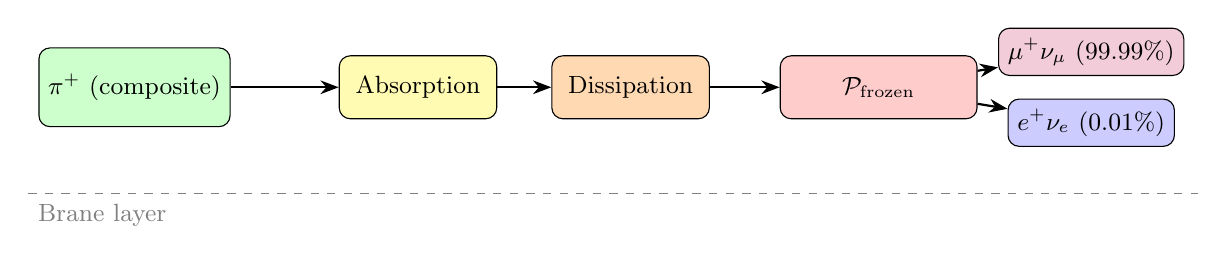
\begin{tikzpicture}[scale=0.9, every node/.style={font=\small}]
    % Pion initial state (composite)
    \node[draw, rounded corners, fill=green!20, minimum width=2cm, minimum height=1cm]
        (pion) at (0,0) {$\pi^+$ (composite)};

    % Absorption stage
    \node[draw, rounded corners, fill=yellow!30, minimum width=2cm, minimum height=0.8cm]
        (abs) at (4,0) {Absorption};

    % Dissipation stage
    \node[draw, rounded corners, fill=orange!30, minimum width=2cm, minimum height=0.8cm]
        (diss) at (7,0) {Dissipation};

    % Projection operator
    \node[draw, rounded corners, fill=red!20, minimum width=2.5cm, minimum height=0.8cm]
        (proj) at (10.5,0) {$\mathcal{P}_{\mathrm{frozen}}$};

    % Output channels
    \node[draw, rounded corners, fill=purple!20, minimum width=1.8cm, minimum height=0.6cm]
        (mu) at (13.5,0.5) {$\mu^+\nu_\mu$ (99.99\%)};
    \node[draw, rounded corners, fill=blue!20, minimum width=1.8cm, minimum height=0.6cm]
        (e) at (13.5,-0.5) {$e^+\nu_e$ (0.01\%)};

    % Arrows
    \draw[-{Stealth}, thick] (pion) -- (abs);
    \draw[-{Stealth}, thick] (abs) -- (diss);
    \draw[-{Stealth}, thick] (diss) -- (proj);
    \draw[-{Stealth}, thick] (proj) -- (mu);
    \draw[-{Stealth}, thick] (proj) -- (e);

    % Brane layer indication
    \draw[dashed, gray] (-1.5,-1.5) -- (15,-1.5);
    \node[gray, anchor=west] at (-1.5,-1.8) {Brane layer};
\end{tikzpicture}
\caption{Energy flow in charged pion leptonic decay. The pipeline is
identical to muon/tau decay, with the pion as initial composite state.
The projection operator $\mathcal{P}_{\mathrm{frozen}}$ strongly favors
the $\mu$-channel~[BL].}
\label{fig:pipeline}
\end{figure}

\subsection{Energy Bookkeeping (Qualitative)}

\begin{table}[h]
\centering
\caption{Energy ledger for $\pi^+ \to \ell^+\nu_\ell$ (qualitative, no fitted values)}
\label{tab:energy-ledger}
\begin{tabular}{lll}
\toprule
\textbf{Stage} & \textbf{Energy Location} & \textbf{Tag} \\
\midrule
Initial & Composite binding (brane-layer) & [P] \\
Absorption & Transferred to dissipation modes & [P] \\
Dissipation & Redistributed among brane modes & [P] \\
Release & $\ell^+$ kinetic + $\nu_\ell$ kinetic & [Dc] \\
\midrule
Bulk leakage & Suppressed (brane-dominant) & [P] \\
\bottomrule
\end{tabular}
\end{table}

\noindent\textbf{Ledger conservation:} Total energy $m_\pi c^2$ is conserved
through all stages. The ``suppressed bulk leakage'' assumption~[P] ensures
that energy remains on the brane layer until release through allowed channels.

\subsection{Key Difference from Leptonic Decays}

In muon and tau decay, the initial state is a \emph{fundamental} brane-dominant
mode. In pion decay, the initial state is a \emph{composite} brane-dominant
excitation. The pipeline structure is the same; the input ontology differs.

% ============================================================
\section{Helicity Suppression}
\label{sec:helicity}
% ============================================================

\subsection{Standard Model Scaling [BL]}

The Standard Model predicts~\cite{PDG2024}:
\begin{equation}
\Gamma(\pi^+ \to \ell^+\nu_\ell) \propto m_\ell^2 \left(1 - \frac{m_\ell^2}{m_\pi^2}\right)^2
\label{eq:sm-scaling}
\end{equation}
This gives BR($\mu$)/BR($e$) $\approx (m_\mu/m_e)^2 \times (\text{phase space})
\approx 8100$, matching observation~[BL].

The physical origin in SM: the pion has spin-0, so the $\ell^+\nu_\ell$ pair
must have total spin-0. Angular momentum conservation forces a helicity
mismatch for the charged lepton. Lighter leptons have smaller ``wrong helicity''
amplitude, suppressed by $m_\ell$.

\subsection{EDC Projection Mechanism [P]/[OPEN]}

\begin{postulate}[Projection Mechanism for Helicity Suppression]
\label{post:projection-mechanism}
In the EDC framework, the frozen projection operator
\begin{equation}
\mathcal{P}_{\mathrm{frozen}} = \mathcal{P}_{\mathrm{energy}} \circ
\mathcal{P}_{\mathrm{mode}} \circ \mathcal{P}_{\mathrm{chir}}
\label{eq:projection-stack}
\end{equation}
includes a chiral filter $\mathcal{P}_{\mathrm{chir}}$ that acts on
both the decaying composite and the outgoing lepton~[P]/[OPEN].

The filter preferentially allows channels where the outgoing charged
lepton can support the required chirality configuration on the brane
boundary. The mismatch scales with the lepton mass parameter that
characterizes chirality mixing.
\end{postulate}

\noindent\textbf{Physical narration:}
\begin{quote}
\emph{5D cause:} The brane boundary conditions impose chirality
constraints on allowed final states.\\
\emph{Brane response:} The chiral filter $\mathcal{P}_{\mathrm{chir}}$
projects out configurations with insufficient chirality overlap.\\
\emph{3D output:} Observers see $\mu$-channel dominance because the
heavier muon has larger chirality overlap with the pion's release
configuration.
\end{quote}

\subsection{Explicit Derivation Status [OPEN]}

\begin{remark}[Derivation Gap]
\label{rem:derivation-gap}
Deriving the $m_\ell^2$ scaling from explicit boundary-condition
computation remains \textbf{[OPEN]}. Required steps:
\begin{enumerate}
    \item Specify the pion's brane-layer wavefunction (composite structure).
    \item Compute the overlap integral with outgoing lepton modes.
    \item Show that the overlap scales as $m_\ell$ (giving $m_\ell^2$ in rate).
\end{enumerate}
Until this is done, we treat the $m_\ell^2$ scaling as~[BL] and the
projection mechanism as~[P]/[OPEN].
\end{remark}

\begin{tcolorbox}[edcWarning, title={Guardrail: No $m_\ell^2$ Derivation}]
\textbf{This companion does NOT derive the $m_\ell^2$ helicity suppression
factor.} We accept it as a baseline fact~[BL] and show that the EDC
chiral-filter hypothesis is \emph{qualitatively consistent} with the
observed $\mu$-dominance. The explicit boundary-condition computation
that would produce $m_\ell^2$ is flagged~\textbf{[OPEN]}.
\end{tcolorbox}

% ============================================================
\section{Existence and Stability}
\label{sec:stability}
% ============================================================

Why does the pion exist as a metastable object with $\tau_\pi \approx 26$~ns?

\begin{postulate}[Metastability Mechanism]
\label{post:metastability}
The pion is metastable because~[P]/[OPEN]:
\begin{enumerate}
    \item \textbf{Brane localization:} The junction-pair (or equivalent
          composite) is confined to the brane layer by a localization
          potential (spectral gap).
    \item \textbf{Suppressed release:} The only allowed release channels
          ($\ell^+\nu_\ell$) require ``unwinding'' the composite through
          the frozen projection, which is kinematically constrained.
    \item \textbf{No bulk escape:} Direct bulk dissipation is suppressed
          for brane-dominant composites (same as for leptons).
\end{enumerate}
\end{postulate}

\noindent\textbf{Physical narration:}
\begin{quote}
\emph{5D cause:} The brane layer has a spectral gap that traps
composite excitations.\\
\emph{Brane response:} The composite remains localized until it can
release through allowed leptonic channels.\\
\emph{3D output:} Observers detect a particle with finite lifetime
$\tau_\pi \approx 26$~ns~[BL].
\end{quote}

\begin{remark}[No Mass Derivation]
\label{rem:no-mass}
We do \textbf{not} attempt to derive $m_\pi = 140$~MeV from first
principles. This requires a complete theory of quark/defect binding
in the 5D framework, which is~\textbf{[OPEN]}.
\end{remark}

% ============================================================
\section{Allowed Output Sets}
\label{sec:outputs}
% ============================================================

\begin{definition}[Allowed Outputs for $\pi^+$ Decay]
\label{def:allowed-outputs}
The allowed output set for $\pi^+$ leptonic decay is~[Dc]:
\begin{equation}
\mathcal{A}_{\pi^+} = \{(\mu^+, \nu_\mu), (e^+, \nu_e)\}
\end{equation}
Both channels satisfy:
\begin{itemize}
    \item Charge conservation: $+1 \to +1 + 0$
    \item Lepton number: $0 \to (-1)_{\ell^+} + (+1)_{\nu_\ell} = 0$
    \item Energy-momentum: $m_\pi c^2 > m_\ell c^2 + 0$ (kinematically allowed)
    \item Spin: $0 \to \frac{1}{2} + \frac{1}{2}$ (total spin-0 possible)
\end{itemize}
\end{definition}

\begin{table}[h]
\centering
\caption{Pion leptonic channels: experimental vs.\ EDC framing}
\label{tab:channels}
\begin{tabular}{llll}
\toprule
\textbf{Channel} & \textbf{BR (Exp) [BL]} & \textbf{EDC Status} & \textbf{Tag} \\
\midrule
$\pi^+ \to \mu^+\nu_\mu$ & $99.99\%$ & Allowed; projection-favored & [Dc] \\
$\pi^+ \to e^+\nu_e$ & $0.01\%$ & Allowed; projection-suppressed & [Dc] \\
$\pi^+ \to \gamma + X$ & --- & Requires photon ontology & [OPEN] \\
\bottomrule
\end{tabular}
\end{table}

% ============================================================
\section{Chiral Filter Hook}
\label{sec:chiral}
% ============================================================

The chiral projection $\mathcal{P}_{\mathrm{chir}}$ is hypothesized to
arise from brane boundary conditions~[P]/[OPEN]. For pion decay, the
relevant constraint is:

\begin{quote}
\emph{The spin-0 pion must release into a lepton-neutrino pair with
total spin-0. The chiral filter preferentially selects configurations
where the charged lepton's helicity mismatch is minimized—favoring
heavier leptons.}
\end{quote}

\noindent This is qualitatively consistent with the SM helicity suppression,
but the explicit boundary-condition derivation is~[OPEN].

\subsection{Universal Hypothesis}

We hypothesize that the same $\mathcal{P}_{\mathrm{chir}}$ acts in all
weak decays (muon, tau, pion, neutron)~[P]/[OPEN]. If true, this would
unify the selection-rule structure across the EDC weak program.

% ============================================================
\section{Falsifiability Guardrails}
\label{sec:falsifiability}
% ============================================================

Companion P makes no numerical predictions. The following structural
claims are falsifiable:

\begin{enumerate}
    \item \textbf{Ontology:} If the pion's 5D structure is shown to be
          bulk-dominant (not brane-dominant), the ontology postulate~[P] fails.
    \item \textbf{Pipeline:} If pion decay requires a fundamentally
          different mechanism than absorption$\to$dissipation$\to$release,
          the framework generalization fails.
    \item \textbf{Selection rules:} If allowed channels violate the
          $\mathcal{A}_{\pi^+}$ set (e.g., $\pi^+ \to \gamma\gamma$
          becomes dominant over leptonic), the selection rules fail.
    \item \textbf{Helicity suppression:} If future EDC derivation of
          $\mathcal{P}_{\mathrm{chir}}$ predicts $e$-dominance over $\mu$,
          the chiral-filter mechanism fails.
    \item \textbf{Ledger consistency:} If energy bookkeeping cannot close
          (i.e., $m_\pi c^2 \neq E_{\ell} + E_\nu$ within experimental
          precision), the ledger conservation assumption fails.
    \item \textbf{Universality:} If the chiral filter must be different
          for pions than for leptons (M, T), the universal hypothesis fails.
\end{enumerate}

\begin{tcolorbox}[edcGuardrail, title={What Would Falsify Companion P?}]
Any of the above six conditions, if demonstrated experimentally or
theoretically, would require revision or abandonment of the claims
made in this companion. We do \textbf{not} claim immunity to falsification.
\end{tcolorbox}

% ============================================================
\section{Open Problems}
\label{sec:open}
% ============================================================

\begin{enumerate}
    \item \textbf{Derive $m_\pi$ from 5D binding}~[OPEN]: What determines
          $m_\pi \approx 140$~MeV?
    \item \textbf{Derive $\tau_\pi$ from first principles}~[OPEN]: Why
          $\tau_\pi \approx 26$~ns?
    \item \textbf{Derive $m_\ell^2$ scaling from BC}~[OPEN]: Show that
          boundary conditions produce the helicity suppression factor.
    \item \textbf{Junction-pair micro-ontology}~[OPEN]: Is the defect--antidefect
          picture correct? How does color confinement map to 5D?
    \item \textbf{Neutral pion $\pi^0 \to \gamma\gamma$}~[OPEN]: Requires
          photon ontology.
    \item \textbf{Pion-nucleon interactions}~[OPEN]: How do pions couple
          to bulk-core junctions (neutrons/protons)?
\end{enumerate}

% ============================================================
\section{Conclusion}
\label{sec:conclusion}
% ============================================================

Charged pion decay is the first \emph{hadron$\to$lepton injection test}
of the EDC thick-brane microphysics framework. We model the pion as a
brane-dominant composite excitation~[P], distinct from fundamental
leptons and from bulk-core junctions.

The absorption$\to$dissipation$\to$release pipeline applies without
modification. The dominant $\mu$-channel and suppressed $e$-channel
are consistent with the frozen-projection + chiral-filter mechanism,
treating helicity suppression as a baseline fact~[BL] with a qualitative
EDC interpretation~[P]/[OPEN].

\textbf{No numerical fits are claimed.} The $m_\ell^2$ scaling derivation
from boundary conditions remains~[OPEN].

\subsection{Why Companion P Matters}

The pion is the \emph{lightest hadron} and the first composite object
to undergo the hadron$\to$lepton transition in the EDC weak program.
Its successful accommodation by the absorption$\to$dissipation$\to$release
pipeline demonstrates that:
\begin{enumerate}
    \item The pipeline is \textbf{not restricted to fundamental particles}---it
          generalizes to composite brane excitations.
    \item The \textbf{ontological distinction} (fundamental vs.\ composite,
          brane-dominant vs.\ bulk-core) is physically meaningful within EDC.
    \item The chiral filter hypothesis gains support from a \textbf{third
          particle sector} (hadrons), beyond the lepton-only tests (M, T).
\end{enumerate}
This positions the EDC weak program as a candidate unified description
of weak decays across particle types, pending resolution of the [OPEN]
problems listed in \S\ref{sec:open}.

\subsection{Position in the EDC Weak Program}

\begin{table}[h]
\centering
\begin{tabular}{llll}
\toprule
\textbf{Companion} & \textbf{Particle} & \textbf{Ontology} & \textbf{Status} \\
\midrule
N & Neutron & Bulk-core junction & v3.0 \\
M & Muon & Brane-dominant (fundamental) & v0.2 \\
T & Tau & Brane-dominant (higher mode) & v0.1 \\
\textbf{P} & \textbf{Pion} & \textbf{Brane-dominant (composite)} & \textbf{v0.3} \\
\bottomrule
\end{tabular}
\end{table}

% ============================================================
% BIBLIOGRAPHY
% ============================================================
\begin{thebibliography}{9}
\bibitem{PDG2024}
R.~L.~Workman \textit{et al.} (Particle Data Group),
``Review of Particle Physics,''
Prog.\ Theor.\ Exp.\ Phys.\ \textbf{2024}, 083C01 (2024).
\end{thebibliography}

\end{document}
